\section*{Ejercicios}
	
\begin{enumerate}
		
\item En un circuito serie RL con $R=\qty{5}{\ohm}$ y $L=\qty{0.06}{\henry}$, la tensión en bornes de la bobina es $u_L(t)=15\sin(200\,t)\,\si{\volt}$. Determinar:
    \begin{itemize}
    \item La tensión total
    \item Intensidad de corriente
    \item Ángulo de desfase de la intensidad respecto de la tensión
    \item Impedancia del circuito
    \end{itemize}
  \emph{Sol.:\;
    $\overline{Z}_{eq}=5+\mathrm{j}\,12\,\si{\ohm};\;\overline{I}=0.88\phase{-90^\circ}\,\si{\ampere};\;\overline{U}=11.48\phase{-22.5304^\circ}\,\si{\volt};\; \phi=67.4696^\circ$}

\item Una resistencia de \qty{5}{\ohm} y un condensador se unen en serie. La tensión en la resistencia es $u_R(t) = 25 \cdot \sin(2000t + \pi/6)\,\si{\volt}$. Si la corriente está adelantada \ang{60} respecto de la tensión aplicada, ¿cuál es el valor de la capacidad C del condensador?

\emph{Sol.:\;
    $C = \SI[parse-numbers = false]{100\sqrt{3}/3}{\micro\farad}$}
  

\item Para determinar las constantes R y L de una bobina, se conecta en serie con una resistencia de \qty{25}{\ohm} y al conjunto se le aplica una fuente de tensión de \qty{120}{\volt} a \qty{60}{\hertz}. Se miden las tensiones en bornes de la resistencia y de la bobina, obteniendo los valores $U_R = \qty{70.8}{\volt}$ y $U_B = \qty{86}{\volt}$. ¿Cuáles son las constantes de la bobina en cuestión?

  \emph{Sol.:\; $R = \qty{5}{\ohm};\; L = \qty{79.5}{\milli\henry}$}

\item Un circuito serie RLC con $R = \qty{5}{\ohm}$ , $L = \qty{0.02}{\henry}$ y $C=\qty{80}{\micro\farad}$, tiene aplicada una tensión senoidal de frecuencia variable. Determinar los valores de la pulsación $\omega$ para los cuales la corriente:
    \begin{itemize}
    \item Adelanta \qty{45}{\degree} a la tensión
    \item Está en fase con ella
    \item Retrasa \qty{45}{\degree}
    \end{itemize}
  \emph{Sol.:\;
    $\omega=\qty{675.39}{\radian\per\second};\; \omega=\qty{790.57}{\radian\per\second};\;
    \omega=\qty{925.39}{\radian\per\second}$}

\item Determinar el triángulo de potencias de un circuito al que se le
aplica una tensión $u(t)=340 \cdot \cos(\omega t - \pi/3)$ V y
por el que circula una intensidad de corriente
$i(t)= 13.3 \cdot \cos(\omega t-0.85)\,\si{\ampere}$.
  
  \emph{Sol.:\;  P =
    \qty{2217.17}{\watt};\; Q = \qty{-443.03}{\voltampere_r};\; S =
    \qty{2261}{\voltampere} }

\item En el esquema de la figura, los elementos tienen los siguientes valores:
    \begin{align*}
      R_1 &= R_2 = R_3 = \qty{10}{\ohm}\\
      X_1 &= X_2 = \qty{1}{\ohm}\\
      R_L &= X_L = \qty{1}{\ohm}
    \end{align*}
  Sabiendo que $U_{CD} = \qty{200}{\volt}$, se debe calcular:
    \begin{itemize}
    \item Intensidades de corriente $I$, $I_1$, $I_2$ e $I_3$ {en forma
        fasorial}, tomando $U_{CD}$ como referencia de fase
    \item Lectura de los vatímetros $W_1$ y $W_2$
    \end{itemize}
  \begin{center}
    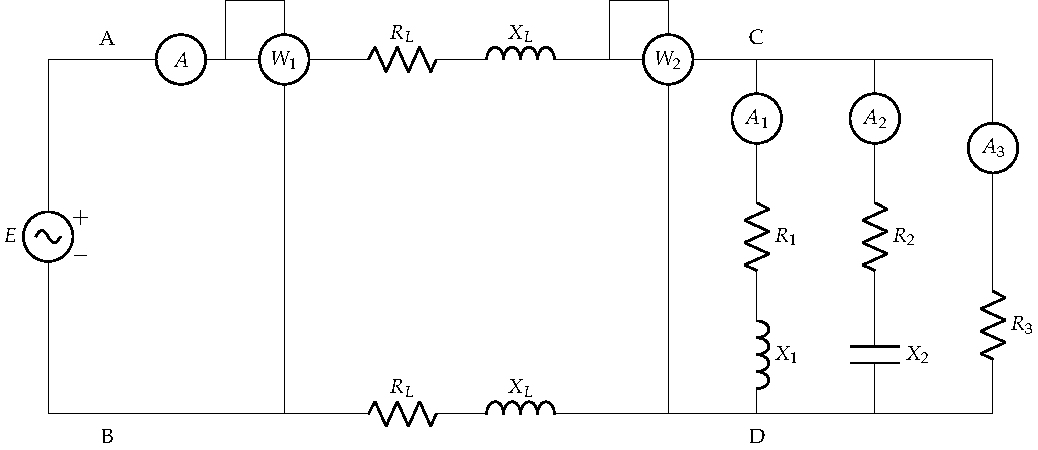
\includegraphics[width=\linewidth]{../figs/ej8_BT2.pdf}
  \end{center}

  \emph{Sol.:\;
    $\overline{I}_1=19.9\phase{-5.7106^\circ}\,\si{\ampere};\;
    \overline{I}_2=19.9\phase{5.7106^\circ}\,\si{\ampere};\;
    \overline{I}_3=20\phase{\ang{0}}\,\si{\ampere};\;\overline{I}=59.6\phase{\ang{0}}\,\si{\ampere};\;W_1=\qty{19024.3}{\watt};\;
    W_2=\qty{11920}{\watt}$}

\item En el circuito de la figura, los amperímetros $A_1$ y $A_2$ marcan $\qty{4.5}{\ampere}$ y $\qty{6}{\ampere}$, respectivamente, el voltímetro, $\qty{150}{\volt}$, y el vatímetro, $\qty{900}{\watt}$. Sabiendo que la frecuencia del generador es de $\qty{250}{\hertz}$ y el f.d.p. de la impedancia $Z$ es de $0.8$ en retraso, calcula:

\begin{itemize}
\item Valores de R, C y Z en forma compleja.
\item La tensión del generador.
\item Triángulo de potencias totales.
\end{itemize}
  \begin{center}
    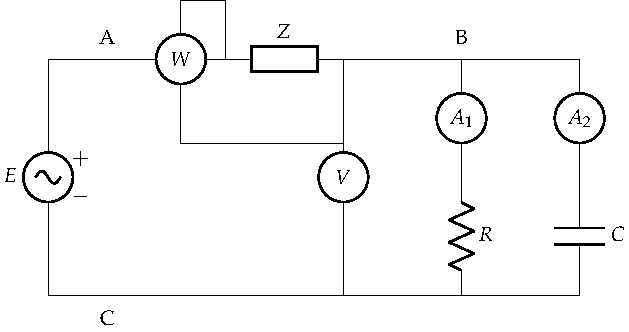
\includegraphics{../figs/ej9_BT2.pdf}
  \end{center}

  \emph{Sol.:\;
    $\overline{R}=33.33\phase{0^\circ}\,\Omega;
    \;\overline{X}_c=-\mathrm{j}\,25\,\Omega;\;\overline{Z}=16+\mathrm{j}\,12\,\Omega;\;\overline{U}_{AC}=212.13\phase{45^\circ}
    \,\si{\volt}; \;\overline{S} = \qty[parse-numbers=false]{1575 - j225}{\voltampere}$}

\item En el circuito de la figura, determinar las lecturas de los aparatos de medida y el balance de potencias activas y reactivas, así como el triángulo global de potencias.\\
Datos: $\; e(t)=100\sqrt{2}\cos(\omega\,t)\,\si{\volt}$;\; $R_1=2\,\Omega$;\;
$R_2=4\,\Omega$;\; $\omega L_1=3\,\Omega$;\; $\omega L_2=4\,\Omega$.

  \begin{center}
    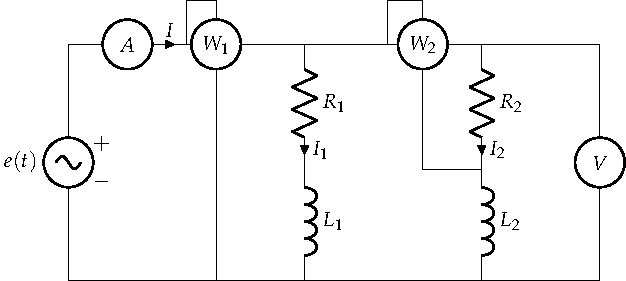
\includegraphics{../figs/ej11_BT2.pdf}
  \end{center}
    
  \emph{Sol.:\;
    $V=\qty{100}{\volt};\; A = \qty{45.20}{\ampere};\; W_1=\qty{2789.35}{\watt};\; W_2= \qty{1250.33}{\watt};\; P_{R1}=\qty{1539.02}{\watt};\; P_{R2}=\qty{1250.33}{\watt};\; Q_{L1}=\qty{2308.52}{\voltamperer};\; Q_{L2}=\qty{1250.33}{\voltamperer};\; P_T=\qty{2789.35}{\watt};\; Q_T=\qty{3558.82}{\voltamperer};\; \overline{S}_T=2789.35+\mathrm{j}3558.82\,\si{\voltampere}$}

\item El circuito de la figura tiene carácter inductivo.  La
  impedancia de la línea es $Z={10\sqrt{2}}{\Omega}$ con
  f.d.p. $\sqrt{2}/2$ en retraso. Tomando como referencia de fases la
  intensidad total $\overline{I}$, se pide calcular:
  \begin{itemize}
  \item Potencia activa y reactiva consumida por $Z$
  \item Expresiones complejas de las intensidades medidas por los
    amperímetros $A$, $A_1$, $A_2$ y $A_3$
  \item Expresiones complejas de las tensiones $\overline{U}_{AB}$,
    $\overline{U}_{AC}$ y $\overline{U}_{CB}$
  \item Valores de $R_1$, $X_1$, $R_2$, $R_3$ y $X_3$
  \end{itemize}
  Datos:
  $A = {5\sqrt{5}}{A};\; A_1 = {5\sqrt{2}}{A};\;A_2 = {5}{A};\;A_3 =
  {\sqrt{10}}{A};\;U_{AB} = {247}{V};\;W_1 = {2350}{W};\;R_1 = R_3$
  \begin{center}
    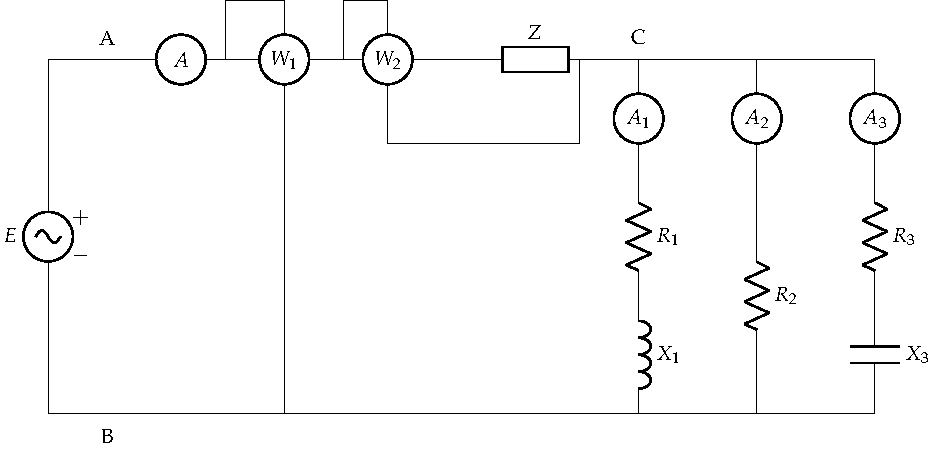
\includegraphics[width=0.8\linewidth]{../figs/ej17_BT2.pdf}
  \end{center}
  \emph{Sol.:
    $P_z=1250\,W;\;Q_z=1250\,VAr;\;\overline{I}=11.18\phase{0^\circ}A;\;
    \overline{I_1}=7.07\phase{-34.6711^\circ}A;\;
    \overline{I_2}=5\phase{10.3289^\circ}A;\;\overline{I_3}=3.16\phase{81.8940^\circ}A;\;
    \overline{U_{AB}}=247\phase{31.6823^\circ}V;\;
    \overline{U_{AC}}=158.11\phase{45^\circ}\,V;\;
    \overline{U_{CB}}=100\phase{10.3289^\circ}
    V;\;R_1=R_3=10\Omega;\;R_2=20\Omega;
    X_1=10\Omega;\;X_3=-30\Omega$}

\item La potencia reactiva del circuito de la figura es
  $\qty{80}{\voltampere_r}$ de tipo capacitivo. La tensión en la
  impedancia Z está en fase con la intensidad $I_1$ y las lecturas de
  los aparatos son $A = \qty{4}{\ampere}$, $V = \qty{50}{\volt}$,
  $W = \qty{200}{\watt}$. Sabiendo que $R_1 = \qty{10}{\ohm}$ y
  $X_2 = \qty{50}{\ohm}$, calcula:

  \begin{enumerate}
  \item Las corrientes $I_1$, $I_2$, $I_3$ en forma fasorial.
  \item Las reactancias $X_1$, $X_3$, y la impedancia $\overline{Z}$.
  \item La fuerza electromotriz $\overline{\epsilon}$.
  \end{enumerate}
  \begin{center}
    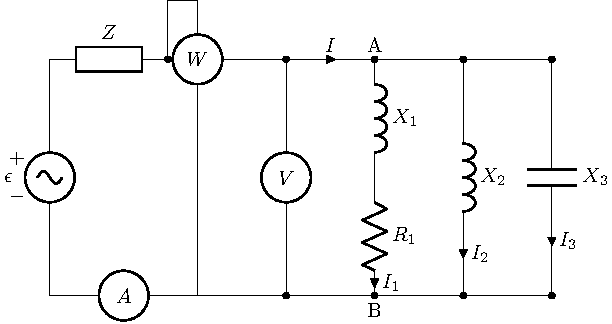
\includegraphics{../figs/BT2_circuitoCapacitivo}
  \end{center}
  \emph{Sol.:\; 
    $\overline{I} =
    4\phase{\ang{0}}\unit{\ampere};
    \overline{I}_1 =
    2\sqrt{5}\phase{\ang{-26.56}}\unit{\ampere}
    ; \overline{I}_2 =
    1\phase{\ang{-90}}\unit{\ampere} ; X_1 =
    \qty{5}{\ohm}; X_3 =
    \qty[parse-numbers=false]{\frac{50}{3}}{\ohm}; \overline{Z} =
    \qty[parse-numbers=false]{10 - j5}{\ohm}$ }

\item Un motor monofásico de $S = {10}{kVA}$ y $fdp = 0.8$ está
  alimentado por una fuente de ${230}{V}$ a $f = {50}{Hz}$.  Calcular:
  \begin{itemize}
  \item El valor eficaz de la corriente absorbida por el motor
  \item La potencia aparente del generador
  \item La capacidad del condensador necesario para compensar el
    factor de potencia a la unidad
  \item El valor eficaz de la corriente absorbida por el conjunto
    condensador-motor
  \item La potencia aparente del generador necesario una vez conectado
    el condensador del tercer apartado
  \item Compara de forma razonada los resultados de los apartados 4 y
    5 con los valores calculados en los apartados 1 y 2
  \end{itemize}
  \emph{Sol.:
    $I= {43.5}{A};\; S_g = {10}{kVA};\;C={361}{\mu F};\, I'=34.78A;\,
    S_g' = {8000}{kVA}$}

\item Un generador de corriente alterna monofásica ($f=\qty{50}{\hertz}$) 
    alimenta a dos cargas a través de una línea de cobre. Esta línea, de resistividad $\rho=\qty{21}{\milli\ohm\milli\meter\squared\per\meter}$, tiene una longitud de $\qty{100}{\meter}$ y una sección de $\qty{16}{\milli\meter\squared}$. Las dos cargas, cuya tensión de alimentación es de $\qty{230}{\volt}$, son dos motores, uno con potencia de $\qty{7}{\kilo\watt}$ y f.d.p. de $0.65$, y otro con una potencia de $\qty{5}{\kilo\watt}$ y f.d.p. de $0.85$. Con esta información, se pide calcular:
    \begin{itemize}
        \item Triángulo de potencias de cada carga y del conjunto de ambas.
        \item Valor eficaz de las corrientes en cada carga y de la corriente   total.
        \item Triángulo de potencias del generador.
        \item Valor eficaz de la tensión en bornes del generador.
        \item Capacidad del condensador a instalar en bornes de las cargas para mejorar el factor de potencia a $0.95$.
        \item Valor eficaz de la corriente entregada por el generador una vez instalado el condensador.
        \item Triángulo de potencias del generador una vez instalado el condensador.
    \end{itemize}
  \emph{Sol.:\;
    $P_1=\qty{7000}{\watt};\;
    Q_1=\qty{8183.91}{\voltampere_r};\;S_1=\qty{10769.23}{\voltampere};\;P_2=\qty{5000}{\watt};\;Q_2=\qty{3098.72}{\voltampere_r};\;S_2=\qty{5882.53}{\voltampere};\;P_T=\qty{12000}{\watt};\;Q_T=\qty{11282.63}{\voltampere_r};\;S_T=\qty{16471.12}{\voltampere};\;
    I_1=\qty{46.82}{\ampere};\;I_2=\qty{25.58}{\ampere};\;I_T=\qty{71.62}{\ampere};\;P_g=\qty{13346.23}{\watt};\;Q_g=\qty{11282.63}{\voltampere_r};\;S_g=\qty{17476.26}{\voltampere};\;U_g=\qty{244.4}{\volt};\; C=\qty{441.66}{\micro\farad};\;I'=\qty{54.92}{\ampere};\;P_g'=\qty{12791.75}{\watt};\;Q_g'=\qty{3944.21}{\voltampere_r};\;S_g'=\qty{13386.02}{\voltampere}$}

\item Un generador de corriente alterna monofásica ($f = {50}{Hz}$)
  alimenta a dos cargas a través de una línea de cobre. Esta línea, de
  resistividad $\rho = {0.017}{\Omega mm^2/m}$, tiene una longitud de
  {40}{m} y una sección de {6}{mm$^2$}. Las dos cargas, cuya tensión
  de alimentación es de {200}{V}, son:
  \begin{enumerate}
  \item Un motor de {7}{kW} con f.d.p. {0,7}.
  \item Un grupo de lámparas fluorescentes con potencia total {200}{W}
    y f.d.p. {0,5}.
  \end{enumerate}
  Se pide:
  \begin{itemize}
  \item Esquema del circuito señalando adecuadamente los elementos,
    corrientes y tensiones
  \item Potencias activa, reactiva y aparente de cada carga
  \item Valor eficaz de las corrientes en cada carga, y de la
    corriente total
  \item Potencia activa y reactiva entregada por el generador
  \item Valor eficaz de la tensión en bornes del generador
  \item Capacidad necesaria a instalar en bornes de las cargas para
    mejorar el factor de potencia de las mismas a la unidad
  \item Valor eficaz de la tensión en bornes del generador, y potencia
    aparente entregada por el mismo una vez instalada la capacidad
    determinada en el apartado anterior
  \end{itemize}
  \emph{Sol.:
    $P_M = {7000}{W};\; Q_M = {7141.43}{VAr};\; S_M ={10000}{VA};\;
    P_F = {200}{W};\; Q_F = {346.41}{VAr};\; S_F ={400}{VA};\;I_M =
    {50}{A};\; I_F = {2}{A};\; I_T = {51.94}{A};\;P_g =
    {7811.50}{W};\; Q_g = {7487.8}{VAr};\; U_g = {208.33}{V};
    C={595.86}{\mu F};\; U_g' = {207.92}{V};\; S_g' = {7485.12}{VA}$ }

\item Un generador de corriente alterna ($f = \SI{50}{\hertz}$)
  alimenta una instalación eléctrica a través de una línea de cobre
  ($\rho = \SI{0.017}{\ohm\milli\meter\squared\per\meter}$) de
  $\SI{25}{\milli\meter\squared}$ de sección. La instalación eléctrica
  está compuesta por un motor de $S_m = \SI{10}{\kilo\voltampere}$ y
  $\mathrm{fdp} = 0.8$, una instalación de alumbrado fluorescente de
  $P_f = \SI{800}{\watt}$ y $\mathrm{fdp} = 0.9$, y diversas cargas
  electrónicas con una potencia conjunta $P_e = \SI{540}{\watt}$ y
  $\mathrm{fdp} = 0.5$ en retraso.

  Suponiendo que las cargas trabajan a su tensión nominal de
  $\SI{230}{\volt}$ y que están situadas a $\SI{100}{\meter}$ del
  generador, calcule:

  \begin{enumerate}
  \item Triángulo de potencias total de las cargas ($P_T$, $Q_T$,
    $S_T$) y factor de potencia.
  \item Valor eficaz de la corriente que circula por la línea.
  \item Potencia disipada en la línea.
  \item Triángulo de potencias del generador ($P_g$, $Q_g$, $S_g$) y
    factor de potencia.
  \item Valor eficaz de la tensión de salida del generador.
  \item Capacidad del banco de condensadores a instalar en bornes de
    la carga necesario para reducir la corriente que circula por la
    línea a un valor de $\SI{45}{\ampere}$.
  \end{enumerate}

  Independientemente del resultado obtenido, suponga que la capacidad
  instalada es $C = \SI{172}{\micro\farad}$. En estas condiciones,
  calcule:
  \begin{enumerate}[resume]
  \item Potencia aparente de las cargas (incluyendo al banco de
    condensadores)
  \item Valor eficaz de la corriente que circula por la línea y
    potencia disipada en la misma.
  \item Triángulo de potencias del generador y factor de potencia.
  \item Tensión de trabajo del generador.
  \end{enumerate}
  \emph{Sol.
    $ S_T = \SI{11868.4}{\voltampere}; I = \SI{51.6}{\ampere}; P_L =
    \SI{362.1}{\watt}; S_g = \SI{12155.4}{\voltampere}; U_g =
    \SI{235.6}{\volt}; C = \SI{172.3}{\micro\farad}; S'_T =
    \SI{10350.1}{\voltampere}; I' = \SI{45}{\ampere}; S'_g =
    \SI{10599.2}{\voltampere}; U'_g = \SI{235.5}{\volt} $}

\item
Calcular la corriente $i(t)$ del circuito de la figura.

  \begin{center}
    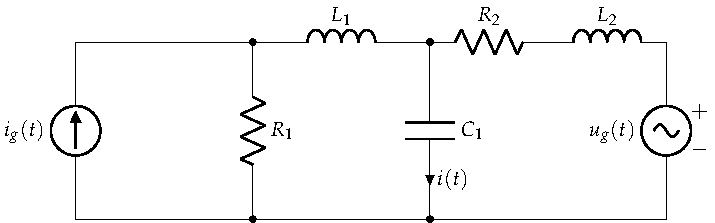
\includegraphics[width=\linewidth]{../figs/BT2_13.pdf}
  \end{center}

Datos: $i_g(t) = 10\sqrt{2}\sin(100t)\unit{\ampere}$; $R_1 = R_2 = \qty{1}{\ohm}$; $L_1 = L_2 = \qty{0.01}{\henry}$; $C_1 = \qty{0.01}{\farad}$; $u_g(t) = 10\sqrt{2}\cos(100t)\unit{\volt}$


  \emph{Sol.: $i(t)=\sqrt{2}\,10\,\cos(100\,t) A$}

\item Del circuito de la figura obtener:
  \begin{itemize}
  \item Expresiones analíticas de las intensidades $i_1(t)$ e $i_2(t)$
  \item Potencia disipada por todas las resistencias
  \end{itemize}

  Datos: $e_g(t)=50\sqrt{2}\sin(1000\,t)$ V; $i_g(t)=10$ A;
  $R_1=R_2=2\Omega$; $R_3=7\Omega$; $L_1=L_2=1$ mH; $L_3=2$ mH
  \begin{center}
    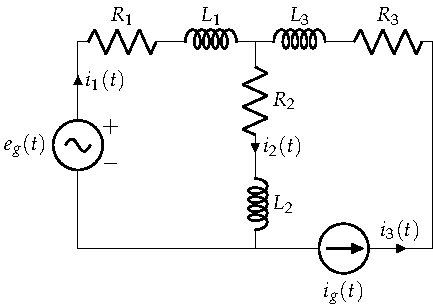
\includegraphics{../figs/ej18_BT2.pdf}
  \end{center}
  \emph{Sol.:
    $i_1(t)= -5+5\sqrt{10}\sin(1000t-0.46) A;\; i_2(t)=
    5+5\sqrt{10}\sin(1000t-0.46) A;\; i_3(t)= 10 A;\; P_T=1300\,W$}

\item En el circuito de la figura determina:
  \begin{itemize}
  \item $u_R(t)$ y $u_L(t)$
  \item Balance de potencias
  \end{itemize}
  Datos:
  $e_a(t) = {3\sqrt{2} \sin(10^3 t)} V;\,e_b(t) = {30\sqrt{2}
    \sin(10^4 t)} V;\,R = {30}{\Omega};\,L = {3}{mH}$
  \begin{center}
    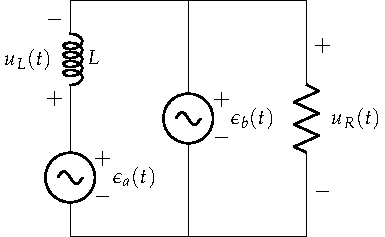
\includegraphics{../figs/superposicion2_ej.pdf}
  \end{center}

  \emph{Sol.:
    $u_R(t) = 30\sqrt{2}\sin(10^4 t) V;\; u_L(t) = 3\sqrt{2}\sin(10^3
    t) - 30\sqrt{2}\sin(10^4 t) V;\; P_R = {30}{W};\; P_\epsilon =
    {30}{W}$}

\item El circuito de la figura se encuentra en régimen
  permanente. Determinar analíticamente la expresión de $i(t)$, así
  como las potencias entregadas por los generadores y disipadas por
  las resistencias $R_1$ y $R_2$.

  Datos:
  $e_1(t) = {50 \sin(1000 t)} V;\; e_2(t) = {30}{V};\; R_1 =
  {6}{\Omega};\; R_2 = {6}{\Omega};\; L = {8}{mH};\; C = {10}{\mu F}$

  \begin{center}
    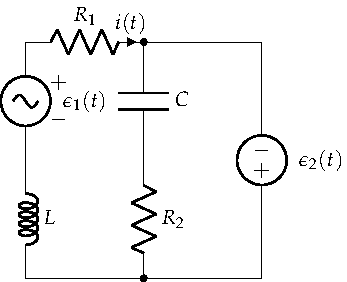
\includegraphics{../figs/superposicion1_ej.pdf}
  \end{center}
  \emph{Sol.:
    $i(t) = 5 + 5\sin(1000t - 0.9273){A};\; P_{R1} = {225}{W}; P_{R2}
    = {0}{W}; P_{\epsilon} = {225}{W}$}

\item   Obtén el generador equivalente de Thévenin del circuito de la figura
  respecto de A y B.

\begin{center}
  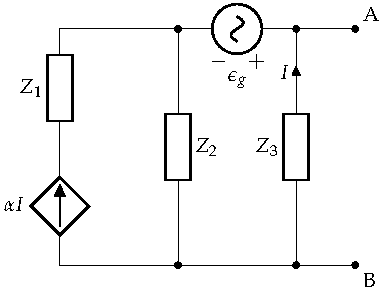
\includegraphics{../figs/Thevenin4}
\end{center}

Datos:
\begin{equation*}
  \overline{\epsilon_g} = \qty[parse-numbers=false]{12 - 16j}{\volt};
  \overline{Z}_1 = \qty[parse-numbers=false]{1 - j}{\ohm};
  \overline{Z}_2 = \qty[parse-numbers=false]{1 + j}{\ohm};
  \overline{Z}_3 = \qty[parse-numbers=false]{5 + 3j}{\ohm}
  \alpha = 2
\end{equation*}
\emph{Sol.
  $ \overline{\epsilon}_{th} = 11.66\phase{\ang{-59.04}}\unit{\volt};
  \overline{Z}_{th} = 0.64 + 0.52j\si{\ohm}$}

\item Obtén el generador equivalente de Thévenin del circuito de la figura respecto de A y B. A partir de este generador, calcula la impedancia a colocar en AB para obtener la máxima potencia, calculando esta potencia.

\begin{minipage}{0.5\textwidth}
\begin{center}
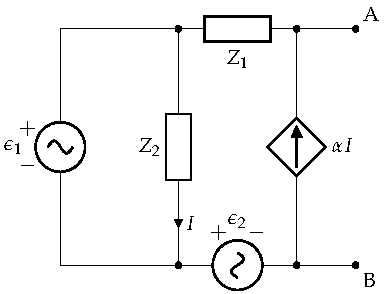
\includegraphics{../figs/Thevenin5}
\end{center}
\end{minipage}
\begin{minipage}{0.5\textwidth}
  \begin{align*}
    \overline{\epsilon_1} &= \SI[parse-numbers=false]{10\phase{0}}{\volt}\\
    \overline{\epsilon_2} &= \SI[parse-numbers=false]{10j}{\volt}\\
    \overline{Z}_1 &= \SI[parse-numbers=false]{4 - 3j}{\ohm}\\
    \overline{Z}_2 &= \SI[parse-numbers=false]{3 + 4j}{\ohm}\\
    \alpha &= 2
  \end{align*}
\end{minipage}

\emph{Sol. $
  \overline{\epsilon}_{th} =  10 - 10j \unit{\volt};
  \overline{Z}_{th} = 4 - 3j \unit{\ohm}
  $}

\end{enumerate}
%%% Local Variables:
%%% mode: latex
%%% TeX-master: "enunciados_ejercicios_TC"
%%% ispell-local-dictionary: "castellano"
%%% End:
